%%%%%%%%%%%%%%%%%%%%%%%%%%%%%%%%%%%%%%%%%
% Short Sectioned Assignment
% LaTeX Template
% Version 1.0 (5/5/12)

%
% This template has been downloaded from:
% http://www.LaTeXTemplates.com
%
% Original author:
% Frits Wenneker (http://www.howtotex.com)
%
% License:
% CC BY-NC-SA 3.0 (http://creativecommons.org/licenses/by-nc-sa/3.0/)
%
%%%%%%%%%%%%%%%%%%%%%%%%%%%%%%%%%%%%%%%%%

%----------------------------------------------------------------------------------------
%	PACKAGES AND OTHER DOCUMENT CONFIGURATIONS
%----------------------------------------------------------------------------------------

\documentclass[paper=a4, fontsize=11pt]{scrartcl} % A4 paper and 11pt font size

\usepackage{graphicx} 
\usepackage{listings}
\usepackage[T1]{fontenc} % Use 8-bit encoding that has 256 glyphs
\usepackage{fourier} % Use the Adobe Utopia font for the document - comment this line to return to the LaTeX default
\usepackage[english]{babel} % English language/hyphenation
\usepackage{amsmath,amsfonts,amsthm} % Math packages
\usepackage{caption}
\captionsetup{font = {scriptsize}}
\usepackage{lipsum} % Used for inserting dummy 'Lorem ipsum' text into the template
\usepackage{subfigure}
\usepackage{latexsym}
\usepackage{sectsty} % Allows customizing section commands
\allsectionsfont{\centering \normalfont\scshape} % Make all sections centered, the default font and small caps
\usepackage{color} %red, green, blue, yellow, cyan, magenta, black, white
\definecolor{mygreen}{RGB}{28,172,0} % color values Red, Green, Blue
\definecolor{mylilas}{RGB}{170,55,241}
\usepackage{float}
\usepackage{fancyhdr} % Custom headers and footers
\pagestyle{fancyplain} % Makes all pages in the document conform to the custom headers and footers
\fancyhead{} % No page header - if you want one, create it in the same way as the footers below
\fancyfoot[L]{} % Empty left footer
\fancyfoot[C]{} % Empty center footer
\fancyfoot[R]{\thepage} % Page numbering for right footer
\renewcommand{\headrulewidth}{0pt} % Remo\label{\label{key}}ve header underlines
\renewcommand{\footrulewidth}{0pt} % Remove footer underlines
\setlength{\headheight}{13.6pt} % Customize the height of the header

\numberwithin{equation}{section} % Number equations within sections (i.e. 1.1, 1.2, 2.1, 2.2 instead of 1, 2, 3, 4)
\numberwithin{figure}{section} % Number figures within sections (i.e. 1.1, 1.2, 2.1, 2.2 instead of 1, 2, 3, 4)
\numberwithin{table}{section} % Number tables within sections (i.e. 1.1, 1.2, 2.1, 2.2 instead of 1, 2, 3, 4)
\newcommand{\mygamma}{\ensuremath{\gamma{}}}
\setlength\parindent{0pt} % Removes all indentation from paragraphs - comment this line for an assignment with lots of text

%----------------------------------------------------------------------------------------
%	TITLE SECTION
%----------------------------------------------------------------------------------------

\newcommand{\horrule}[1]{\rule{\linewidth}{#1}} % Create horizontal rule command with 1 argument of height

\title{	
\normalfont \normalsize 
\textsc{Purdue University} \\ [25pt] % Your university, school and/or department name(s)
\horrule{0.5pt} \\[0.4cm] % Thin top horizontal rule
\huge ECE 637 Laboratory Exercise 8\\ 
\huge Image Halftoning\\% The assignment title
\horrule{2pt} \\[0.5cm] % Thick bottom horizontal rule
}

\author{Tong Shen} % Your name

\date{\normalsize\today} % Today's date or a custom date

\begin{document}

\maketitle % Print the title

%----------------------------------------------------------------------------------------
%	PROBLEM 1
%----------------------------------------------------------------------------------------
\section{Introduction}
Nothing to report for this section. 

\section{Image Fidelity Metrics}
Nothing to report for this section. 

\section{Thresholding and Random Noise Binarization
}

The simplest method of converting a grayscale image to a binary image is by thresholding, it is a two-level (one-bit) quantization process. 
\subsection{Result Risplay}
\begin{figure}[H]
	
	\centering
	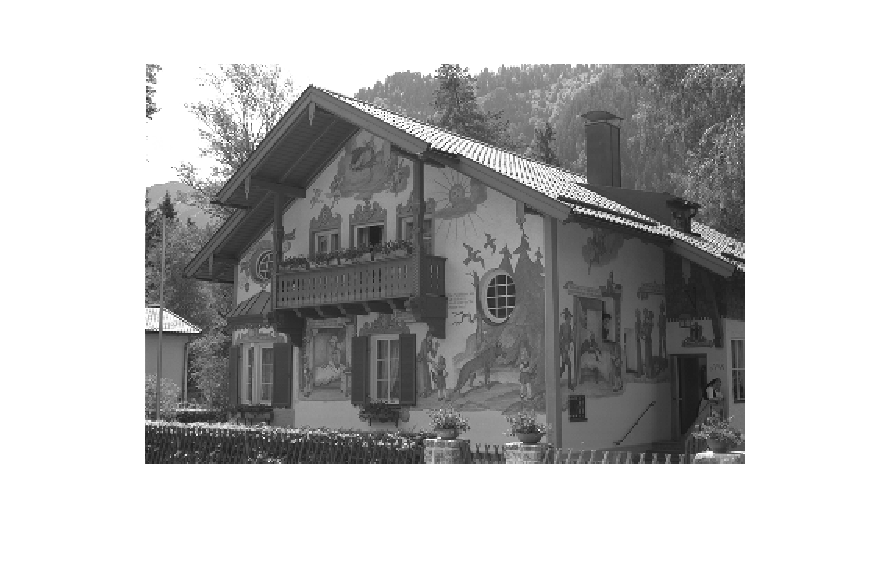
\includegraphics[height = 2.2in]{1.eps}
	\caption{The original image}
	
	
	
\end{figure}
\begin{figure}[H]
	
	\centering
	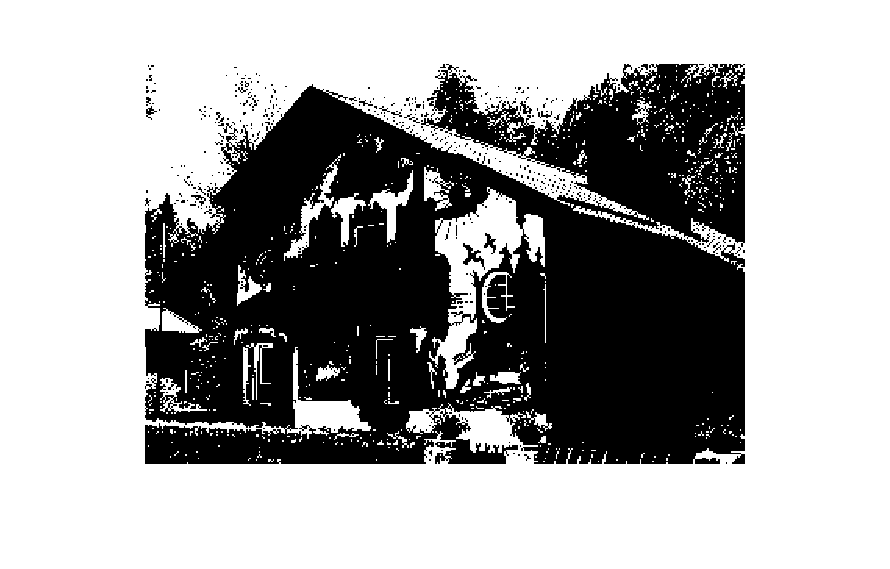
\includegraphics[height = 2.2in]{2.eps}
	\caption{The halftoning image with a threhold of 127}
	
	
	
\end{figure}
And the RMSE and Fidelity Values are as follows:

\begin{equation}
\begin{split}
RMSE = 87.3933\\
Fidelity =    77.3371\\
\end{split}
\end{equation}
\subsection{fidelity.m}
	\lstset{language=Matlab,%
		%basicstyle=\color{red},
		breaklines=true,%
		morekeywords={matlab2tikz},
		keywordstyle=\color{blue},%
		morekeywords=[2]{1}, keywordstyle=[2]{\color{black}},
		identifierstyle=\color{black},%
		stringstyle=\color{mylilas},
		commentstyle=\color{mygreen},%
		showstringspaces=false,%without this there will be a symbol in the places where there is a space
		numbers=left,%
		numberstyle={\tiny \color{black}},% size of the numbers
		numbersep=9pt, % this defines how far the numbers are from the text
		emph=[1]{for,end,break},emphstyle=[1]\color{red}, %some words to emphasise
		%emph=[2]{word1,word2}, emphstyle=[2]{style},    
	}
\begin{lstlisting}[frame=single]

	function d = fidelity(img,b)
	img = 255*(img/255).^2.2;
	
	h = zeros(7);
	temp = 0;
	for i = -3:3
	for j = -3:3
	h(i+4,j+4) = exp(-(i^2+j^2)/4);
	temp = temp + h(i+4,j+4);
	end
	end
	h = h/temp;
	
	img = imfilter(img,h);
	b = imfilter(b,h);
	img = 255*(img/255).^(1/3);
	b = 255*(b/255).^(1/3);
	
	c = sum(sum((img - b).^2));
	[m n] = size(img);
	d = sqrt(c/(m*n));
	
	end
	
	
\end{lstlisting}

\section{ Ordered Dithering}

The goal in halftoning is to give the impression of grayscale tones while using only black
and white pixels. Although the random thresholding technique described before can
produce this effect, it is not often used in real applications since it yields very noisy results.
In this section, we will learn and utilize a better class of halftoning techniques known as ordered
dithering.
\\
The Bayer index matrices of size 2X2 is:
\[
Bayer_{2} = 
\begin{bmatrix}
     1    & 2\\
3     & 0
\end{bmatrix}
\]

The Bayer index matrices of size 4X4 is:
\[
Bayer_{4} = 
\begin{bmatrix}
     5    & 9   &  6  &  10\\
13   &  1  &  14    & 2\\
7   &11  &   4    & 8\\
15  &  3   & 12   &  0
\end{bmatrix}
\]

The Bayer index matrices of size 8X8 is:
\[
Bayer_{8} = 
\begin{bmatrix}
 21  &  37  &  25  &  41 &   22   & 38  &  26   & 42\\
53   &  5   & 57  &   9  &  54    & 6   & 58   & 10\\
29   & 45   & 17  &  33  &  30   & 46  &  18   & 34\\
61   & 13   & 49  &   1  &  62   & 14  &  50  &   2\\
23   & 39   & 27  &  43   & 20   & 36  &  24  &  40\\
55   &  7   & 59  &  11   & 52    & 4   & 56  &   8\\
31   & 47   & 19  &  35   & 28   & 44  &  16  &  32\\
63   & 15   & 51  &   3   & 60   & 12  &  48  &   0
\end{bmatrix}
\]


%------------------------------------------------

\begin{figure}[H]
	
\centering
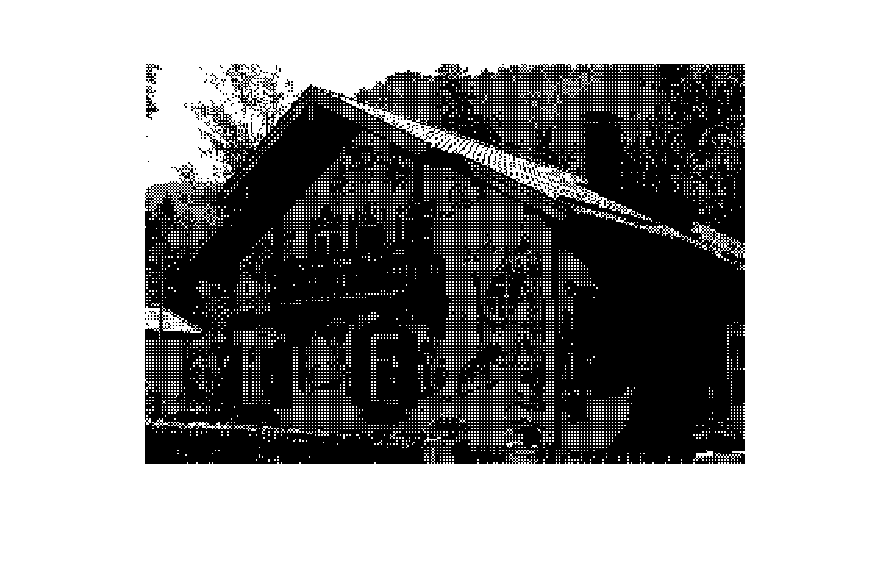
\includegraphics[height = 2.5in]{3.eps}
\caption{Result of Bayer 2X2 matrix}
		
		
\end{figure}
\begin{figure}[H]
	
	\centering
	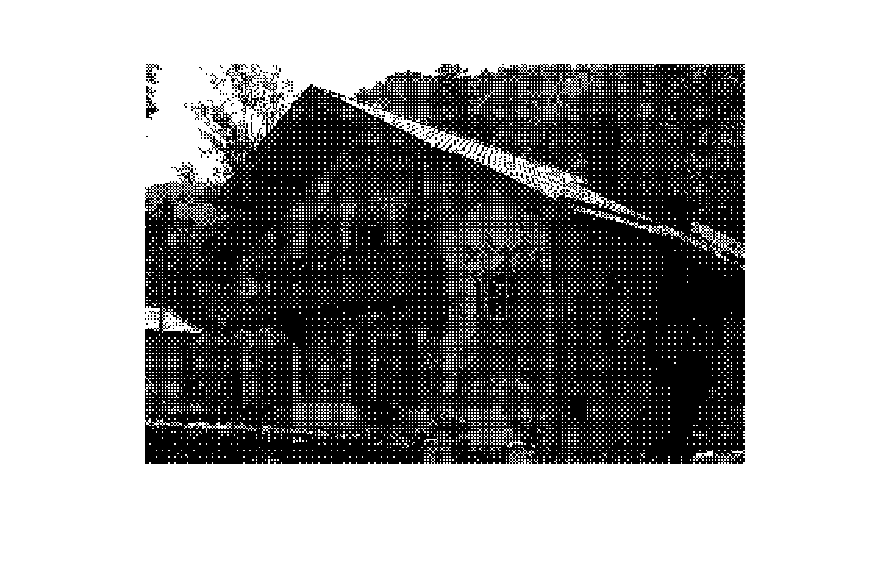
\includegraphics[height = 2.5in]{4.eps}
	\caption{Result of Bayer 4X4 matrix}
	
	
\end{figure}
\begin{figure}[H]
	
	\centering
	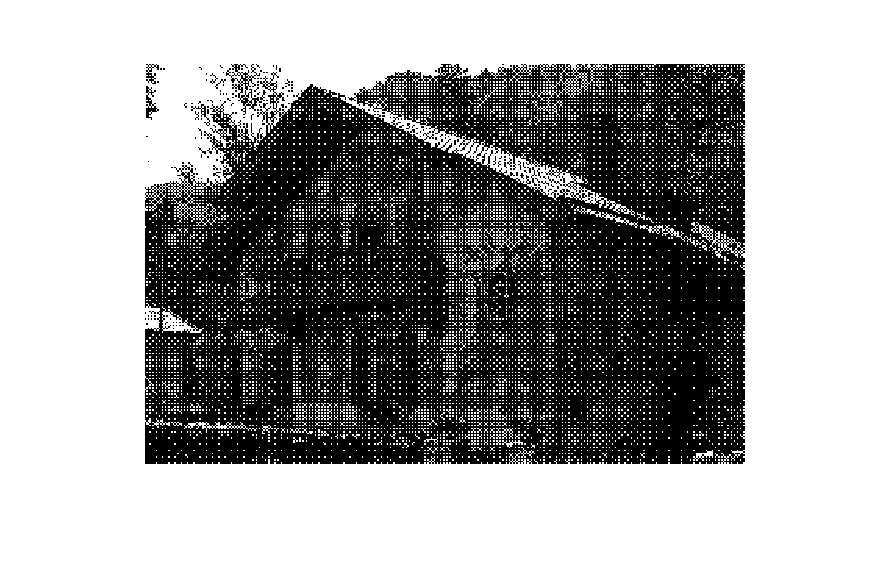
\includegraphics[height = 2.5in]{5.eps}
	\caption{Result of Bayer 8X8 matrix}
	
	
\end{figure}

And the RMSE and Fidelity Values are as follows:

\begin{equation}
\begin{split}
RMSE_{2} = 97.6690\\
Fidelity_2 =    50.0569\\
\end{split}
\end{equation}
\begin{equation}
\begin{split}
RMSE_4 = 101.0069\\
Fidelity_4 =     16.5583\\
\end{split}
\end{equation}
\begin{equation}
\begin{split}
RMSE_8 = 100.9145\\
Fidelity_8 =   14.6918
\end{split}
\end{equation}

\section{Error Diffusion
}

Another class of halftoning techniques are called error diffusion. In this method, the pixels
are quantized in a specific order , and the residual
quantization error for the current pixel is propagated forward to local unquantized
pixels. This keeps the local average intensity of the binary image close to the original
grayscale image.
In this section, we will be to display a calibrated color image from a known illuminant
spectrum and the reflectance coefficients at each point in the image.

\subsection{Code Listing}

\begin{lstlisting}[frame=single]
clc
clear
I0 = imread('house.tif');
I0 = double(I0);
I = (I0/255).^(2.2)*255;
[r,c] = size(I);


for i = 2:r-1
for j = 2:c-1
if I(i,j) > 127
diff = - 255 + I(i,j);
I(i,j) = 255;
else
diff = I(i,j);
I(i,j) = 0;
end
I(i+1,j) = 5/16*diff + I(i+1,j);
I(i,j+1) = 7/16*diff + I(i,j+1);
I(i+1,j+1) = 1/16*diff + I(i+1,j+1);
I(i+1,j-1) = 3/16*diff + I(i+1,j-1);
end
end

imshow(I(2:r-1,2:c-1))
truesize
imwrite(I,'i.tif')

temp = 0;
for i = 1:r
for j = 1:c
temp = temp + (I0(i,j) - I(i,j))^2/(r*c);
end
end
RMSE = sqrt(temp)
fidelity(I0,I)

\end{lstlisting}


\subsection{Result Display}

\begin{figure}[H]
	
	\centering
	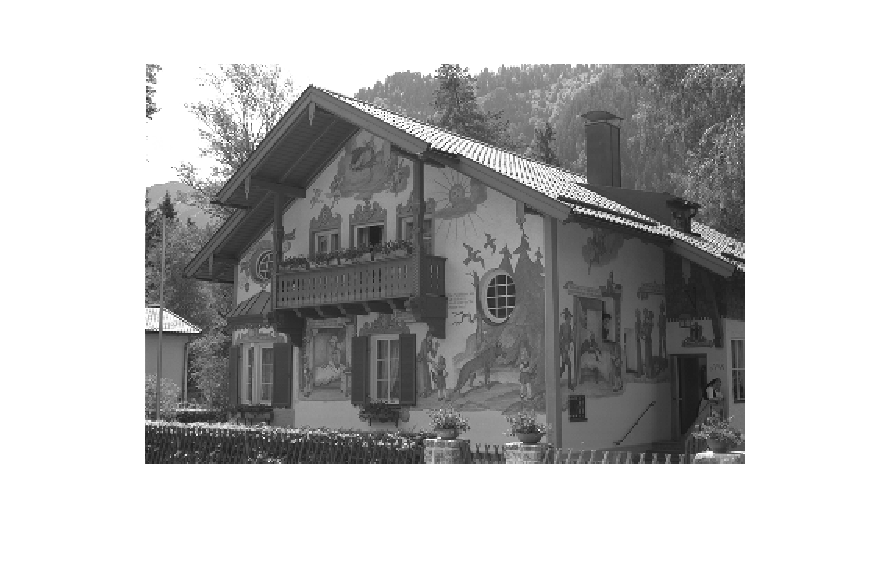
\includegraphics[height = 2.2in]{1.eps}
	\caption{The original image}
	
	
	
\end{figure}
\begin{figure}[H]
	
	\centering
	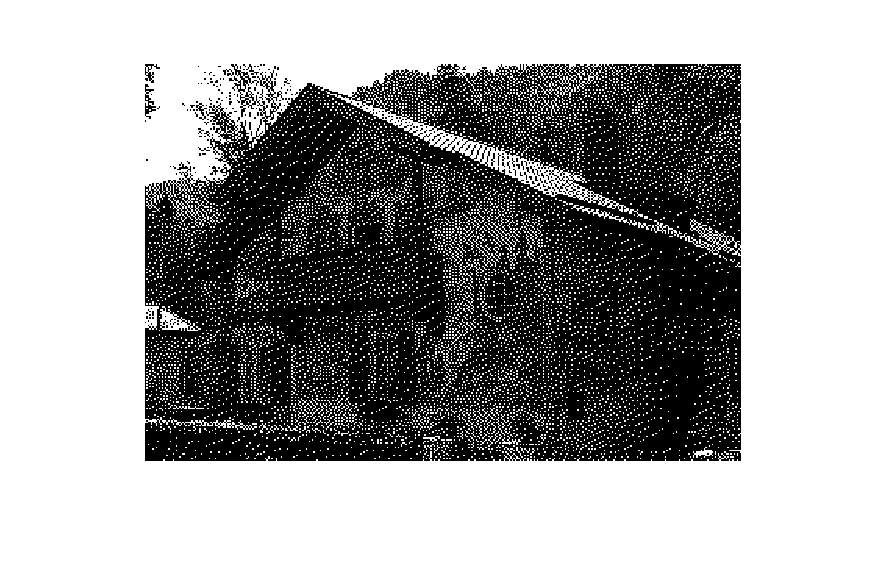
\includegraphics[height = 2.2in]{6.eps}
	\caption{The Error Diffusion Image}
	
	
\end{figure}
And the RMSE and Fidelity Values are as follows:
\centering
\begin{equation}
\begin{split}
RMSE =  98.4725\\
Fidelity =    12.8448
\end{split}
\end{equation}

\subsection{RMSE and fidelity Comparison}
\begin{table}[H]
	\centering  % 表居中
	\begin{tabular}{ |l | c | r|}  % {lccc} 表示各列元素对齐方式,left-l,right-r,center-c
		\hline
		    &RMSE  & Fidelity\\
		    \hline
		Simple Threhold &87.3933 &77.3371\\
			    \hline
		2$\times$2 Ordered Dithering &97.6690 &50.0569\\
			    \hline
		4$\times$4 Ordered Dithering &101.0069 & 16.5583\\
			    \hline
		8$\times$8 Ordered Dithering &100.9145 &14.6918\\
			    \hline
		Error Diffusion &98.4725 &12.8448\\
		   \hline
	\end{tabular}
	\caption{List of Region of Image with different T}
	
\end{table}
\begin{flushleft}
{According to the results, the RMSE values do not change with different method, while the fidelity values change a lot through different method. And we can also conclude that the fidelity values is related to the halftoning quality. The halftoning images with lower fidelity value looks more realistic and have higher resolution. }
\end{flushleft}
\end{document}